\section{Extending Predictions of the BB Model to LLMs} \label{sec:llm}

%\DP{TODO for SONG: rewrite this paragraph}
% \DP{TODO for DRUV: check again after Song finishes}

In this section, we examine extreme-token phenomena in open-source pre-trained LLMs. In \Cref{sub:active_dormant}, we analyze the static behavior of these phenomena in Llama 2-7B-Base \citep{touvron2023llama}, confirming that certain attention heads in LLMs exhibit both active and dormant phases. Notably, we identify a specific head that is active on GitHub samples but dormant on Wikipedia samples, illustrating the \textit{active-dormant mechanism}. In \Cref{sub:olmo_dynamics}, we explore the dynamic behavior of extreme-token phenomena during the pre-training process of OLMo-7B \citep{groeneveld2024olmo}. We show that the attention logits, value state norms, and residual state norms of the sink token(s) in OLMo mirror their behavior in the simpler BB model. Specifically, the simultaneous formation of attention sinks and value state drains gives evidence for the \textit{mutual reinforcement mechanism}.

% It turns out that our exploration into the BB task in \Cref{sec:bb_task} may actually shed light upon the origin of attention sinks, small value states, and massive norms in full-fledged large language models trained on massive amounts of text. To verify this claim, we once again summarize and elaborate the observations we made in the BB task model:
% \begin{enumerate}[leftmargin=2em]
% \setlength\itemsep{0pt}
%     \item The attention sinks and value state drains are external manifestations of the active-dormant mechanism in LLMs. 
%     \item The lower-layer components (e.g., attentions and MLPs) of the LLM contribute to all three extreme-token phenomena.     
%     \item The attention heads go through the attention-increasing and value-state-shrinking phase. They converge to the stable phase, with identical attention logits on the \bos~token. Meanwhile, the residual state norm corresponding to the \bos{} token linearly increase during pre-training.
% \end{enumerate}

% We will confirm each of these observations in this section.\footnote{Here, we mention that in order to achieve this checklist, we had to do a certain amount of translating from the setting of the BB model to the setting of LLMs. For example, the BB model identifies trigger tokens as the (semantically) important tokens in that the model should change behavior after seeing them. In the context of LLMs, almost every token fits this description for a suitable context, but tokens like \bos{} do not. 
% %\tianyu{I think we should say that each token could be trigger or non-trigger, depending on the context? If every tokens are triggers, there's no dormant phase.}
% } Namely, in \Cref{sub:active_dormant} we will confirm point 1; in \Cref{sub:circuits} we confirm point 2; and in \Cref{sub:olmo_dynamics} we confirm point 3.


\subsection{Active-Dormant Mechanism in LLMs}\label{sub:active_dormant}

Our study of the BB model leads to the following prediction about the extreme-token phenomena, which we hypothesize also applies to LLMs:  
\begin{center}
    \textit{Attention heads are controlled by an active-dormant mechanism. Attention sinks and value state drains indicate that an attention head is in dormant phase.}
    %\textit{If all tokens at a head do not have helpful value states for predicting the next token, then attention mass will concentrate on tokens which are generally unhelpful for next-token prediction (like \bos). \sm{Attention heads are controlled by the active-dormant mechanism; attention sinks and value state drains are the dormant phases of attention heads. }}
\end{center}

This hypothesis suggests that in LLMs, attention heads become sinks or not depending on the context: the value vector can be totally non-informative towards picking likely next tokens for token distributions (e.g., tasks) in a particular context but not in others. This is a concrete instantiation vis-a-vis large-scale LLMs of the active-dormant dichotomy in \Cref{sec:bb_task}, where this phenomenon was shown to occur in the context of small next-token predictors and the BB task. 

Accordingly, we strive to find instances of heads in pretrained LLMs which satisfy this principle, i.e., which are dormant on some domains and active on others. In \Cref{fig:dormant_heads_domain_dependent}, we show a particular attention head -- Layer 16 Head 25 of Llama 2-7B-Base \citep{touvron2023llama} --- which has an extremely clear active-dormant distinction across two distinct contexts (e.g., tokens from RedPajama \citep{together2023redpajama} drawn from the GitHub subset versus the Wikipedia subset). While there are many such attention heads which are context-dependent --- we provide some in \Cref{sec:more_heads} --- we demonstrate this one because the conditions under which it is active are simple and interpretable, while others have more involved or complex criteria to become active. We observe that this attention head is \textit{dormant} (i.e., an attention sink) on samples from Wikipedia, which more closely resemble prose, and \textit{active} (i.e., not an attention sink) on samples from Github, which more closely resemble code. We also observe that this attention head, in general, contributes significantly to the performance of the model on code sequences, but has negligible impact on the performance of the model on prose sequences (\Cref{fig:github_wikipedia_zero_out}). This is a further justification, from a practical perspective, of why this head is sometimes dormant and sometimes active --- in some contexts we can ablate it from the model entirely with no effect, but in other contexts ablating the head leads to huge performance drops. %\footnote{Llama 2-7B-Base has two sink tokens (\bos~and one more) in its attention sink heads, while Llama 3.1-8B-Base only has one (\bos). We discuss a potential reason in \Cref{sub:multiple_sinks_discussion}. \sm{Why we put this remark here?}} \sm{Talk about other heads also has dormant and active phase, though not interpretable. Ablation figures in appendix. } \DP{@SM: the first part is already in the paragraph.} \sm{It would be good to link to figures for other heads. } \DP{sure will add to appendix, and comment out this comments when done}
We include more detail in \Cref{sec:circuit}, where we extract a circuit for extreme-token phenomena in order to analyze the dormant-active mechanism and its interaction with the semantics of the input tokens.

\begin{figure}
    \centering
    \begin{subfigure}[t]{0.5\textwidth}
        \centering
        \caption{\small Attention weights for GitHub/Wikipedia data.}% \sm{Maybe 2 by 2? }}
        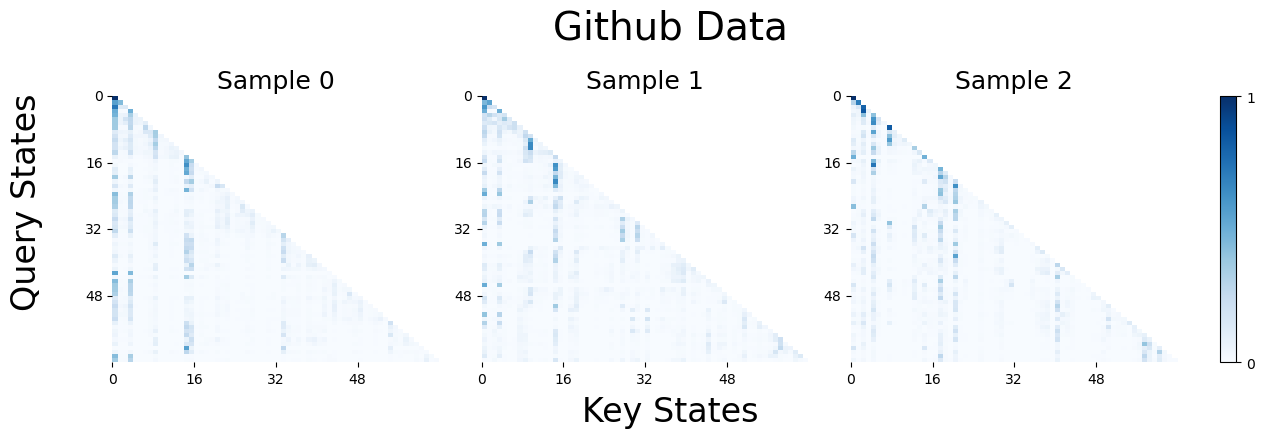
\includegraphics[width=\textwidth]{Figures/L16_H25/attn_weights_l16h25_github_revised.png}
        
        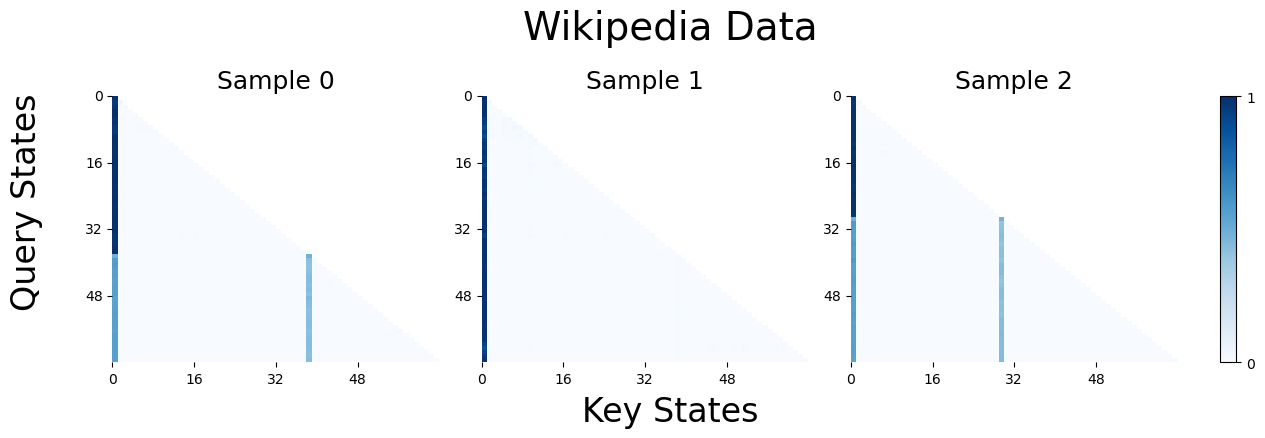
\includegraphics[width=\textwidth]{Figures/L16_H25/attn_weights_l16h25_wikipedia_revised.png}
        \label{fig:github_wikipedia_weights}
    \end{subfigure}
    \hfill
    \begin{subfigure}[t]{0.44\textwidth}
        \caption{\small Zero-out-head intervention outcomes.}
        \label{fig:github_wikipedia_zero_out}
        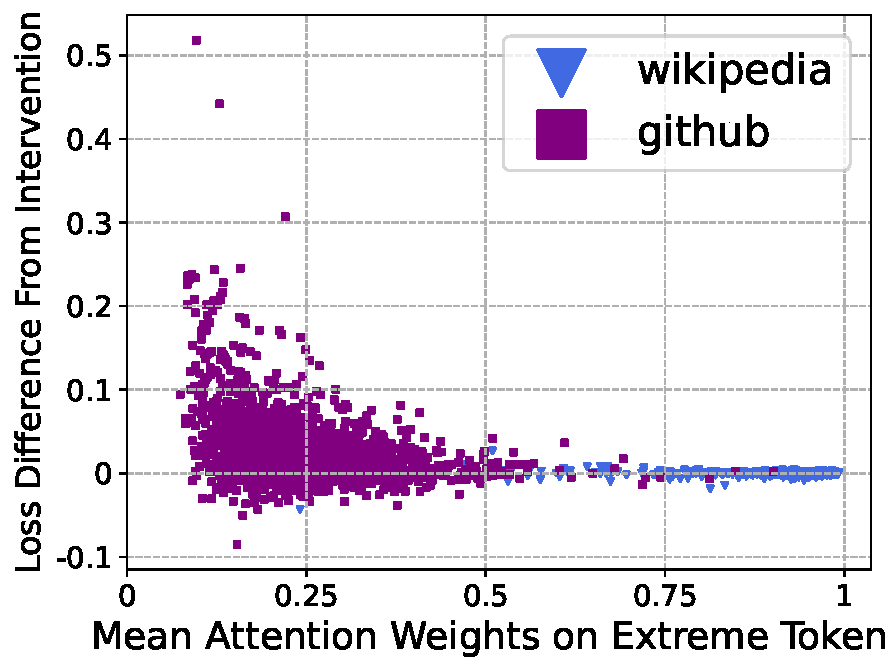
\includegraphics[width=\textwidth]{Figures/BBM/LLM_interventions.pdf}
    \end{subfigure}
    \vspace{-1.5em}
    %\includegraphics[width=0.5\linewidth]{}
    \caption{\small \textbf{Attention heads in LLMs are active on some domains and dormant on others.} For example, on Llama 2-7B-Base, we identify that Layer 16 Head 25 is active when the context contains many tokens related to programming, and dormant in other contexts such as prose. We use RedPajama-1T \citep{together2023redpajama} Wikipedia and Github subsets for our data in this figure, truncating all samples to 64 tokens for demonstration purposes. \textit{Left:} Sample weights from four randomly selected samples from each domain. \textit{Right:} Result of an intervention study, i.e., change in cross-entropy of the input sequence when the attention head's output (concretely, the value states for this head) is manually set to zero, across sequences in both domains. We observe that the model's performance, measured by cross-entropy, strongly depends on the output of the attention head on coding data.
    % heads are sinks in one domain and not others (Llama 2 7B L16H25, Github vs Wikipedia) \DP{TODO...}
    % \DP{Plan: two figures. Left: attn sink visualization for Github on left and Wikipedia (4x4 (adjust to be visually appealing) samples visualize L16H25). Right: causal intervention, zeroing out head vs cross entropy delta taken across many samples from Github and Wikipedia.}
    }
    \label{fig:dormant_heads_domain_dependent}
\end{figure}


\subsection{Training Dynamics of Extreme-Token Phenomena in LLMs}\label{sub:olmo_dynamics}


Our study of the BB model leads to the following prediction about the dynamical behavior of the extreme-token phenomena, which we hypothesize also applies to LLMs:  
\begin{center}
    \textit{The attention heads go through a attention-increasing and value-state-shrinking phase. They then go into a stable phase, with identical attention logits on the \bos~token. Meanwhile, the residual state norm of the \bos{} token linearly increases during pre-training.}
\end{center}

% We confirm these predictions below, thus demonstrating the overall validity of the BB task as a model for extreme token phenomena in LLMs. 
We confirm these predictions below. To observe the training dynamics of a large-scale LLM, we use the setup of OLMo-7B-0424 \citep{groeneveld2024olmo} (henceforth just referred to as OLMo), who have open-sourced weights at several steps during their training run. For our analysis, we inspect OLMo at a variety of training steps: every 500 steps throughout the first 10,000 steps, then 25,000 steps, then 50,000 steps, then every 50,000 steps until 449,000 steps (which is roughly the end of their training). Again, we use the input ``Summer is warm. Winter is cold.''.\footnote{Note that OLMo does not have a \bos{}~token, but attention sinks still form in the majority of heads. In particular, the first token behaves similarly to an attention sink. We discuss this in \Cref{sub:fixed_bos}.} Notice that in this prompt, token \(3\), namely ``.'', is not very semantically meaningful; it becomes a sink token along with token \(0\) (c.f. \Cref{sub:active_dormant}, \Cref{sec:circuit}, \Cref{sub:fixed_bos}).

In \Cref{fig:olmo_predictions_phase0}, we confirm that attention heads go through an attention-increasing and value-state-shrinking phase, and that the residual state norm of the \bos{} token increases linearly during pre-training. We show that, at Layer 24 of OLMo, the average attention on extreme tokens (token \(0\) and token \(3\)) increases rapidly at the beginning of training and converges to a constant, while the value state norms of extreme tokens decrease rapidly. Also, the residual states of extreme tokens also increase linearly, while the rest quickly converge. In \Cref{fig:olmo_predictions_phase1} we show that attention heads converge to a stable phase, and that all logits corresponding to the first token's value states (i.e., all tokens' value of \(\mathrm{logit}_{0}\), except possibly the value of \(\mathrm{logit}_{0}\) corresponding to token \(0\) itself) have similar distributions. These confirm our dynamics insights from the BB model (c.f. \Cref{figure:verify-assumptions}). %\sm{These echos the findings from the BB model. Link figure 3b here. }

\begin{figure}[thp]
    \centering
    \begin{subfigure}[t]{0.32\textwidth}
        \centering 
        \caption{\small Attention sink dynamics (L24).}
        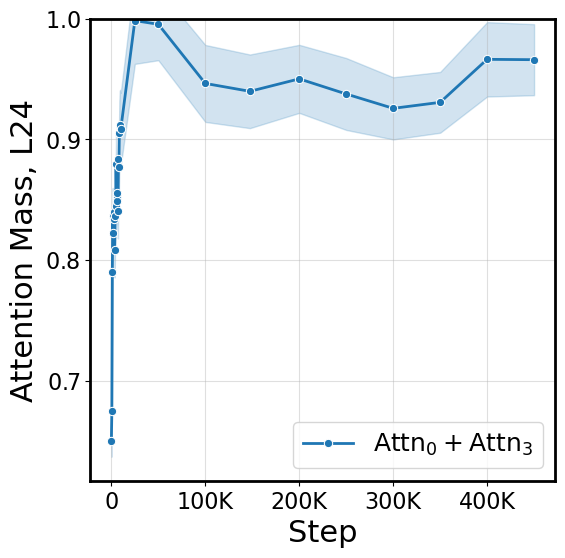
\includegraphics[width=\textwidth]{Figures/olmo/olmo_sink.png}
        \label{fig:olmo_sink}
    \end{subfigure}
    \begin{subfigure}[t]{0.32\textwidth}
        \centering 
        \caption{\small Value state dynamics (L24).}
        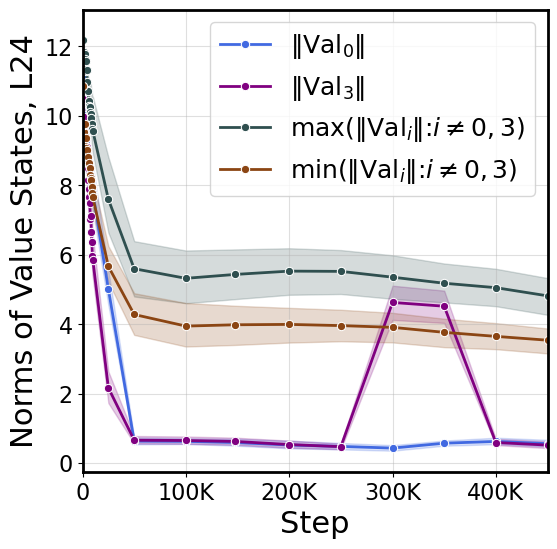
\includegraphics[width=\textwidth]{Figures/olmo/olmo_value_states.png}
    \end{subfigure}
    \begin{subfigure}[t]{0.32\textwidth}
        \centering 
        \caption{\small Residual state dynamics (L24).}
        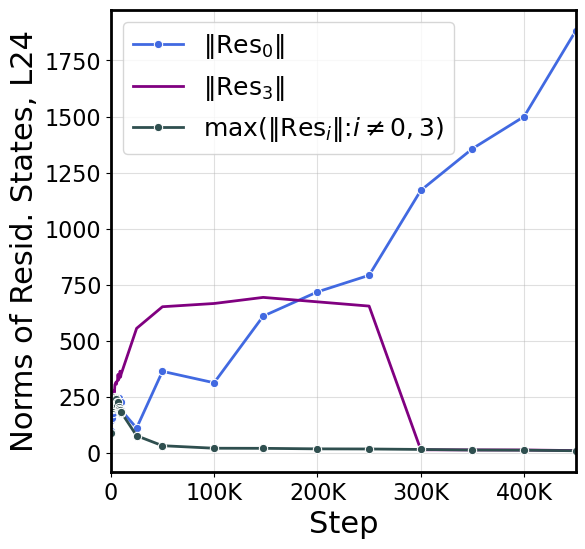
\includegraphics[width=\textwidth]{Figures/olmo/olmo_massive_norms.png}
    \end{subfigure}
    \vspace{-2em}
    \caption{\small \textbf{Attention-increasing and value state-decreasing phase, and residual state norms.} \textit{Left (a):} We plot the total attention mass on extreme tokens \(0\) and \(3\) at Layer 24 and averaged over all attention heads, during OLMo training. We observe that it increases rapidly and then maintains its value in \([0.9, 1]\) for the rest of training, which is in line with our predictions. \textit{Middle (b):} We plot the norm of each token's value state at Layer 24 during training, averaged over all heads. We observe that the value states of all tokens shrink initially and then converge, while the value states of the extreme tokens shrink to much lower than all other tokens. \textit{Right (c):}  We plot the norm of each token's residual state at Layer 24 during training. We observe that the residual state of token \(0\) increases linearly in magnitude during training.}
    \label{fig:olmo_predictions_phase0}
\end{figure}

\begin{figure}[thp]
    \centering
    \hfill
    \begin{subfigure}[t]{0.32\textwidth}
        \centering 
        \caption{\small Logit dynamics (L24).}
        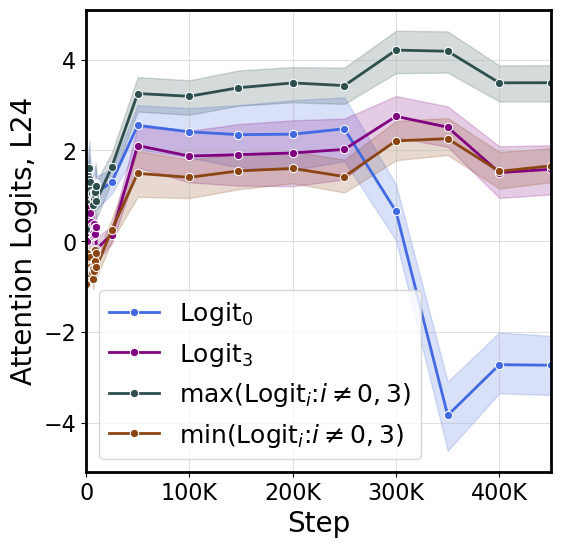
\includegraphics[width=\textwidth]{Figures/olmo/olmo_logits.png}
        \label{fig:attention_logits_olmo_dynamic}
    \end{subfigure}
    \hfill
    \begin{subfigure}[t]{0.32\textwidth}
        \centering 
        \caption{\small Logit statics (L24).}
        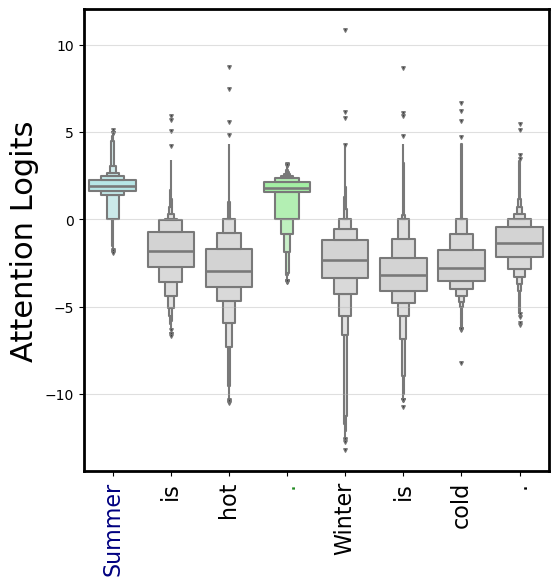
\includegraphics[width=\textwidth]{Figures/olmo/olmo_logits_static.png}
        \label{fig:attention_logits_olmo_static}
    \end{subfigure}
    \hfill
    \phantom{.}
    \vspace{-2em}
    \caption{\small \textbf{Stable phase.}  \textit{Left (a):} We plot the normalized attention logits of all tokens' query states against token \(0\)'s key state during training. We observe that the logits of all non-extreme tokens' query states against token \(0\)'s key state in OLMo's Layer 24 are stable for a large fraction of the training run, after an initialization period. This echoes the stable phase prediction made in the BB model in \Cref{sec:bb_task}. Note that this prediction makes no guarantees about the logit corresponding to the zeroth query token and zeroth key token, which will be set to \(1\) by the softmax and so its behavior is irrelevant for prediction. Also note that we use normalization, similar to \Cref{sec:bb_task}, to make all terms comparable; namely we have \(\mathrm{logit}_{i} = \langle \query_{i}, \key_{0}\rangle - \mathtt{mean}_{j}(\langle \query_{i}, \key_{j}\rangle)\). \textit{Right (b):} For this experiment, we generate \(128\) randomly sampled test tokens with IDs from \(100\) to \(50000\) in the OLMo tokenizer. We append each token separately to the test phrase ``Summer is warm. Winter is cold.'', creating \(128\) different samples, which we feed to the LLM to record the model behavior. We plot the distribution of (un-normalized) dot products \(\langle \query_{\mathrm{test}}, \key_{j}\rangle\) across all heads at Layer 24 and all test tokens. We observe that logits of all regular tokens have very similar distributions, and the distributions of the logits corresponding to extreme tokens \(0\) and \(3\) are also similar. This confirms the hypothesis that at the end of training, attention heads converge to the stable phase, with similar logits on extreme tokens.}
    \label{fig:olmo_predictions_phase1}
\end{figure}



% Outline:
% \begin{itemize}
%     \item OLMo value states at a middle layer are roughly constant over time except for bos token and first delimiter
%     \item Massive norm keeps increasing over time 
%     \item Attention sink occurs very rapidly and stays constant over time
% \end{itemize}

% \begin{figure}
%     \centering
%     %\includegraphics[width=0.5\linewidth]{}
%     \caption{Training dynamics of value states, massive norm, and attention sink via OLMo
%     \DP{TODO: for attention logits plot, put linear plot for first 10k epochs (halfway through axis) and log plot for remaining epochs; do the same for value states; plot multiple heads for value plot}}
%     \label{fig:enter-label}
% \end{figure}












